\section{Realisering og test}
\label{sec:research}

Punktprøvingsfrekvensen $f_s$ er satt til 6,4 kHz. Dermed blir spesifikasjonene som plottet i tabell \ref{tab:spec}. 

\begin{table}[ht]
    \caption{Filterspesifikasjoner}
    \centering
    \begin{tabular}{|l|l|l|}
        \hline
        Spesifikasjon & Formel                              & Verdi        \\ \hline
        $f_s$         &                                     & 6400Hz       \\ \hline
        B             & $\frac{f_s}{2}$                     & 3200Hz       \\ \hline
        $f_c$         & $\geq\frac{3}{8}f_s$                & $\geq$2400Hz \\ \hline
    \end{tabular}
    \label{tab:spec}
\end{table}

Ved å ta i bruk formlene gitt i seksjon \ref{sec:concept} blir beregninene som vist i tabell

\begin{table}[hbt]
    \centering
    \caption{Beregninger.}
    % \setlength\extrarowheight{9pt}
    \begin{large}
    \begin{tabular}{|l|l|l|}
        \hline
        Størrelse   & Formel                                              & Måltall og enhet          \\ \hline
        A           & $10^{\frac{A[dB]}{20}}$                             & $\approx0.3162$           \\ \hline
        n           & $\frac{1}{2}\frac{ln(A^{-2}-1)}{ln(\frac{f}{f_c})}$ & $\approx3.81\rightarrow4$ \\ \hline
        R           &                                                     & $1k\Omega$                \\ \hline
        $\zeta_1$   & tatt fra tabel \ref{tab:polpar}                     & 0.92388                   \\ \hline
        $\zeta_2$   & tatt fra tabel \ref{tab:polpar}                     & 0.38268                   \\ \hline
        $\omega_0$  & $2\pi f_c$                                          & $15079.64\frac{rad}{s}$   \\ \hline
        $\tau_{11}$ & $\frac{1}{\omega_0 \zeta_1}$                        & $71.77\mu s$              \\ \hline
        $\tau_{12}$ & $\frac{1}{\omega_0^2 \tau_{11}}$                    & $61.27\mu s$              \\ \hline
        $\tau_{21}$ & $\frac{1}{\omega_0 \zeta_2}$                        & $173.29\mu s$             \\ \hline
        $\tau_{22}$ & $\frac{1}{\omega_0^2 \tau_{21}}$                    & $25.38\mu s$              \\ \hline
        $C_{11}$      & $\frac{\tau_{11}}{R}$                               & $71.77nF$              \\ \hline
        $C_{12}$      & $\frac{\tau_{12}}{R}$                               & $61.27nF$              \\ \hline
        $C_{21}$      & $\frac{\tau_{21}}{R}$                               & $173.29nF$             \\ \hline
        $C_{22}$      & $\frac{\tau_{22}}{R}$                               & $25.38nF$              \\ \hline
        \end{tabular}
    \end{large}
    \label{tab:calculations}
    \end{table}

Den realiserte er illustrert i figur \ref{fig:01realised}. Merk at verdiene ikke er det samme som på tabell \ref{tab:calculations} da det er små avvik i kondensatorene, men til tross for det så er avviket relativt lavt.

\begin{figure}[!hbt]
	\centering
	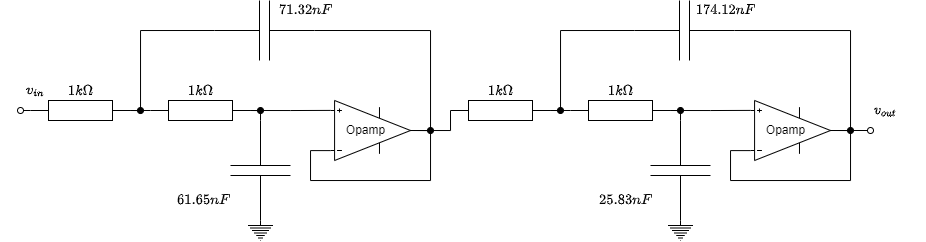
\includegraphics[scale=0.45]{./Images/03Research/01realisertkrets.png}
	\caption{Realisert krets med verdier.}
	\label{fig:01realised}
\end{figure}

Med denne kretsen ble frekvensresponsen lik figur \ref{fig:02frekvensresponsrealisert}.

\begin{figure}[!hbt]
	\centering
	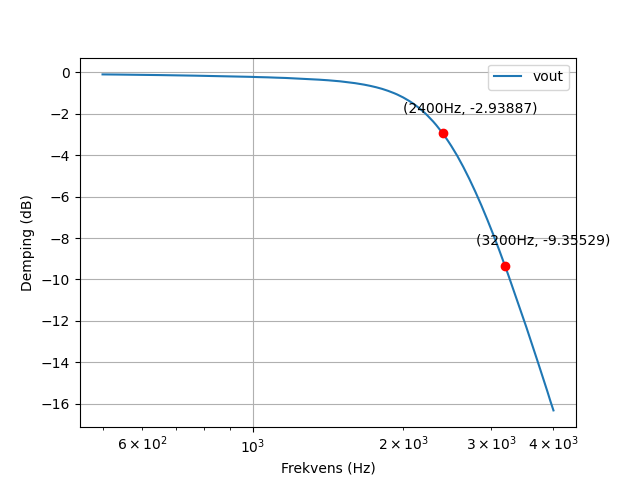
\includegraphics[scale=0.45]{./Images/03Research/02frekvensrespons.png}
	\caption{Frekvensrespons for realisert Anti-alias-filter.}
	\label{fig:02frekvensresponsrealisert}
\end{figure}

Det observeres at med disse komponentene så blir kravet om at knekkfrekvensen skal være $f_c\geq2400Hz$ oppfyllt, men ikke kravet om at dempingen ved $B=3200Hz$ er lavere enn 10dB. Ved å legge til 2,13 nF slik at $C_{22} = 27.96$ blir frekvensresponsen lik figur \ref{fig:02frekvensresponsrealisert2}.

\begin{figure}[!hbt]
	\centering
	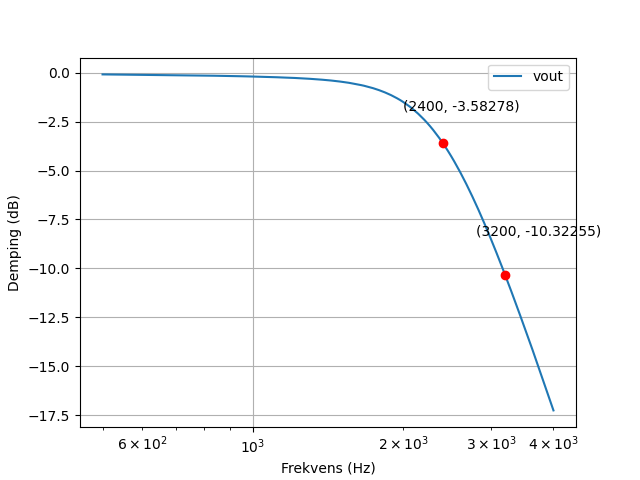
\includegraphics[scale=0.45]{./Images/03Research/02frekvensrespons2.png}
	\caption{Frekvensrespons for realisert Anti-alias-filter med  $C_{22}=27.96$.}
	\label{fig:02frekvensresponsrealisert2}
\end{figure}

Til tross for at det er relativt små avvik på realiserte kondensator verdier og beregnede kondensator verdier så blir ikke begge kravene oppfylt, dette kan skyldes små avvik som støy fra pc-en og spenningsforsyning eller avvik i komponentene.

Det kan vurderes å øke ordenen på systemet i et forsøk om å få oppfylt kravene at knekkfrekvensen skal være $f_c\geq2400Hz$ og samtidig at dempingen ved $B=3200Hz$ blir lavere enn 10dB, men som beskrevet i seksjon \ref{sec:Nødvendig_orden}, så blir ikke brattheten noe serlig større ved en stor orden.

\begin{figure}[!hbt]
	\centering
	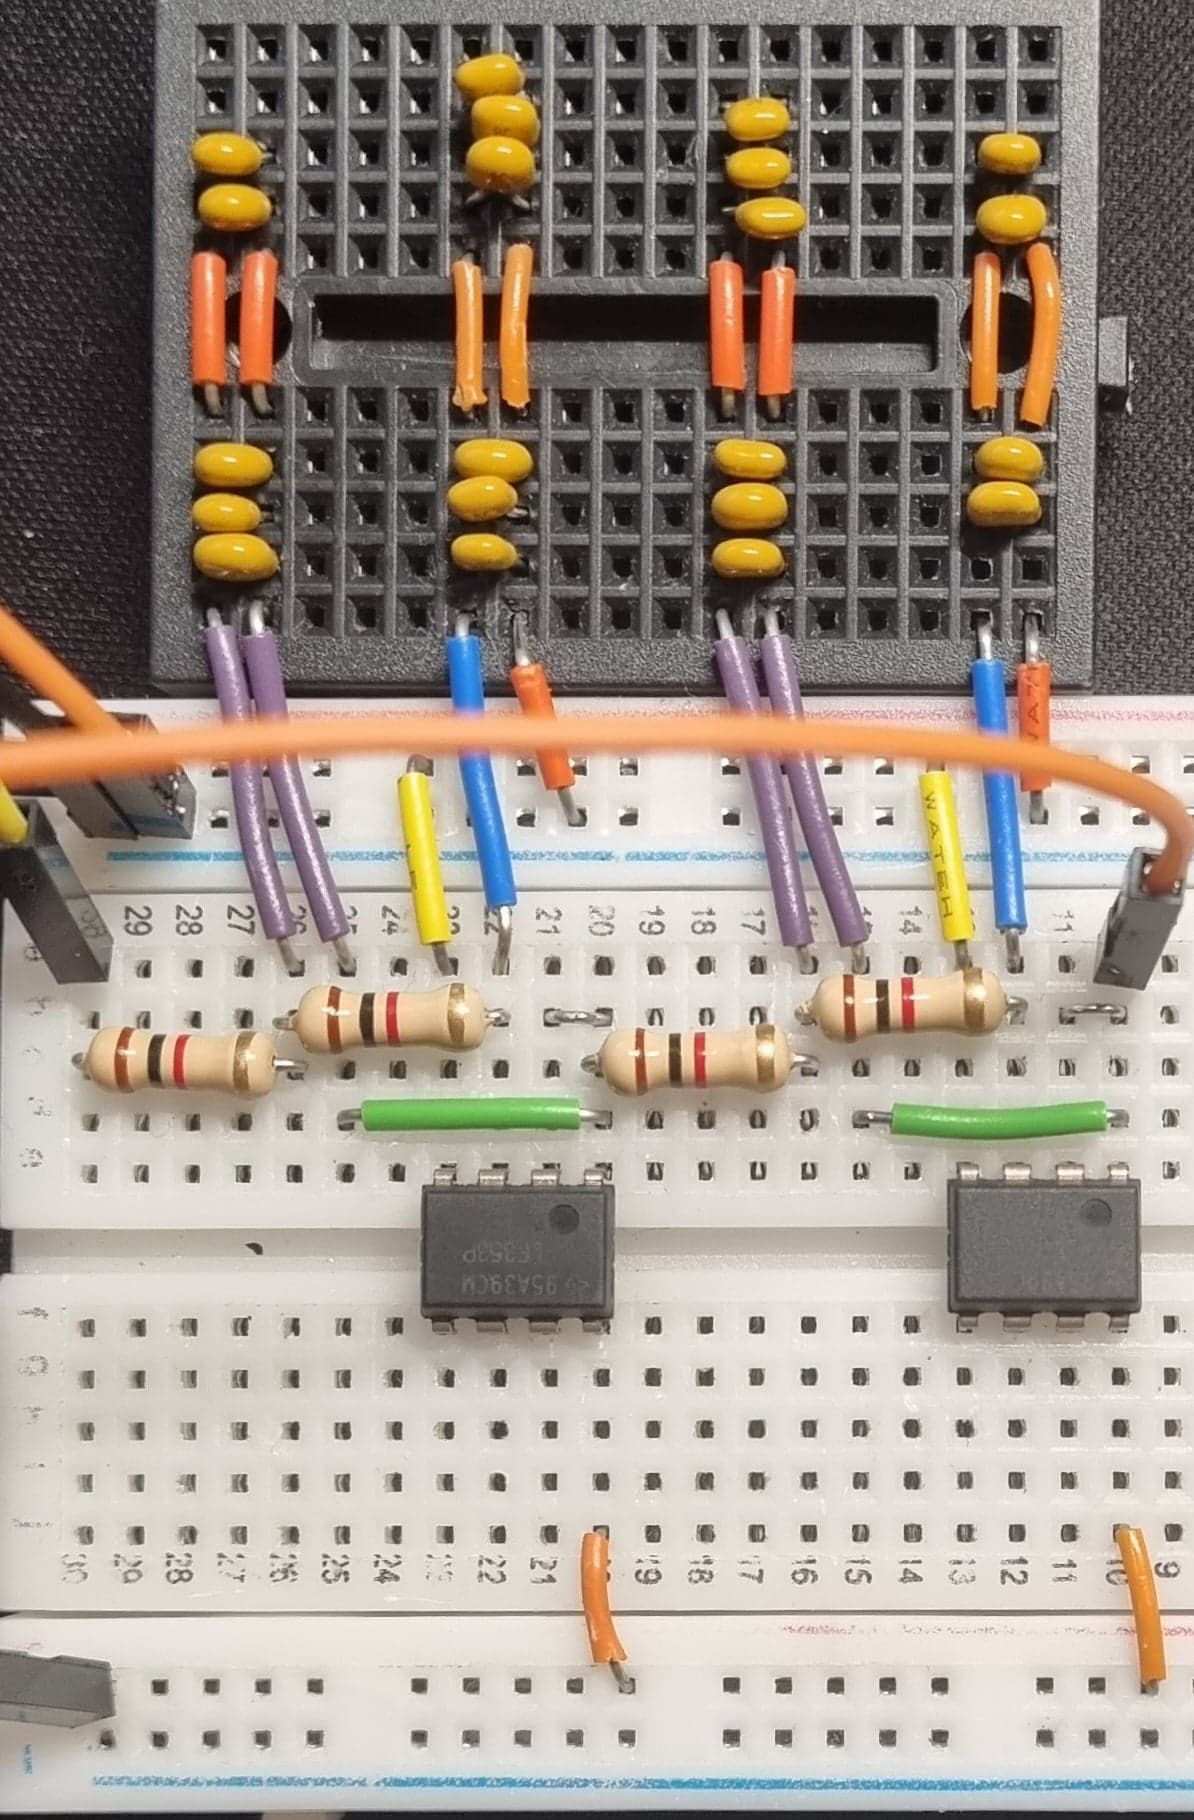
\includegraphics[scale=0.1]{./Images/03Research/03}
	\caption{Fysisk realisert krets.}
	\label{fig:03}
\end{figure}

\begin{equation}
    \Sigma
\end{equation}